%
% related-work.tex
%
% Copyright (C) 2023 by Gabriel Mariano Marcelino.
%
% Towards the Conception of GNSS Networks Based on Small Satellites
%
% This work is licensed under the Creative Commons Attribution-ShareAlike 4.0
% International License. To view a copy of this license,
% visit http://creativecommons.org/licenses/by-sa/4.0/.
%

%
% \brief Related work slides.
%
% \author Gabriel Mariano Marcelino <gabriel.mm8@gmail.com>
%
% \version 1.0.0
%
% \date 2023/09/07
%


\begin{frame}{Related Work}

    \begin{itemize}
        \item Consolidated networks
        \vspace{0.3cm}
        \item Experimental networks
    \end{itemize}

\end{frame}

\begin{frame}{Related Work}

    \begin{itemize}
        \item Global networks:
            \begin{itemize}
                \item GPS
                \item GLONASS
                \item Galielo
                \item BDS
            \end{itemize}
        \item Local networks:
            \begin{itemize}
                \item QZSS
                \item IRNSS
                \item KPS
            \end{itemize}
    \end{itemize}

\end{frame}

\begin{frame}{GPS}

    \begin{itemize}
        \item American network
        \vspace{0.2cm}
        \item Global coverage
        \vspace{0.2cm}
        \item Composed by 24 satellites
        \vspace{0.2cm}
        \item Orbit: MEO ($\cong$ 20,000 km)
        \vspace{0.2cm}
        \item First GNSS system (operational in 1995)
    \end{itemize}

\end{frame}

\begin{frame}{GLONASS}

    \begin{itemize}
        \item Russian network
        \vspace{0.2cm}
        \item Global coverage
        \vspace{0.2cm}
        \item Composed by 24 satellites
        \vspace{0.2cm}
        \item Orbit: MEO ($\cong$ 19,000 km)
        \vspace{0.2cm}
        \item Available for worldwide use in 1995
    \end{itemize}

\end{frame}

\begin{frame}{Galileo}

    \begin{columns}[t]
        \begin{column}[t]{0.5\textwidth}
            \begin{itemize}
                \item European network
                \vspace{0.2cm}
                \item Global coverage
                \vspace{0.2cm}
                \item Composed by 30 satellites
                \vspace{0.2cm}
                \item Orbit: MEO
                \vspace{0.2cm}
                \item Robust ground infrastructure
                \vspace{0.2cm}
                \item Operational in 2016
            \end{itemize}
        \end{column}
        \begin{column}[t]{0.6\textwidth}
            \begin{figure}[!ht]
                \begin{center}
                    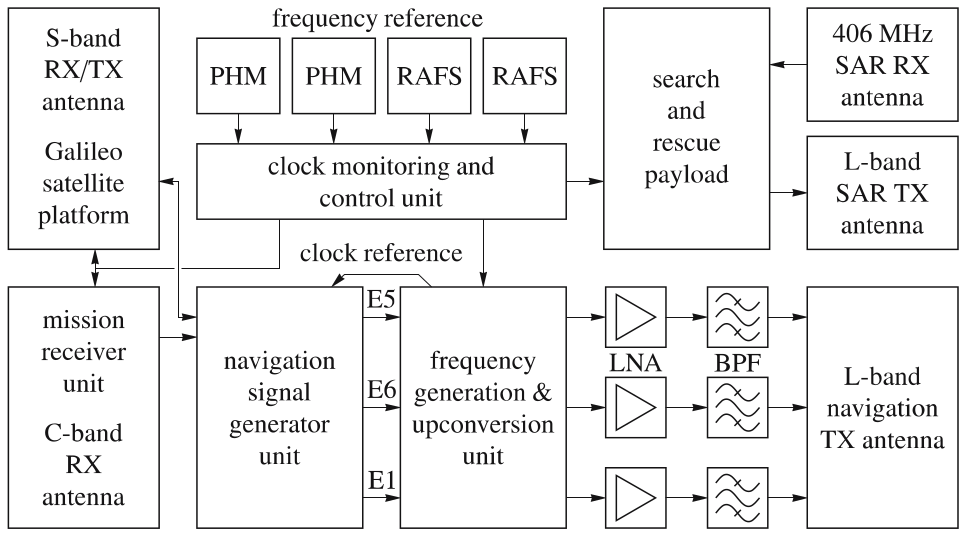
\includegraphics[width=0.9\columnwidth]{figures/galileo-satellite-bd}
                \end{center}
            \end{figure}

            \begin{figure}[!ht]
                \begin{center}
                    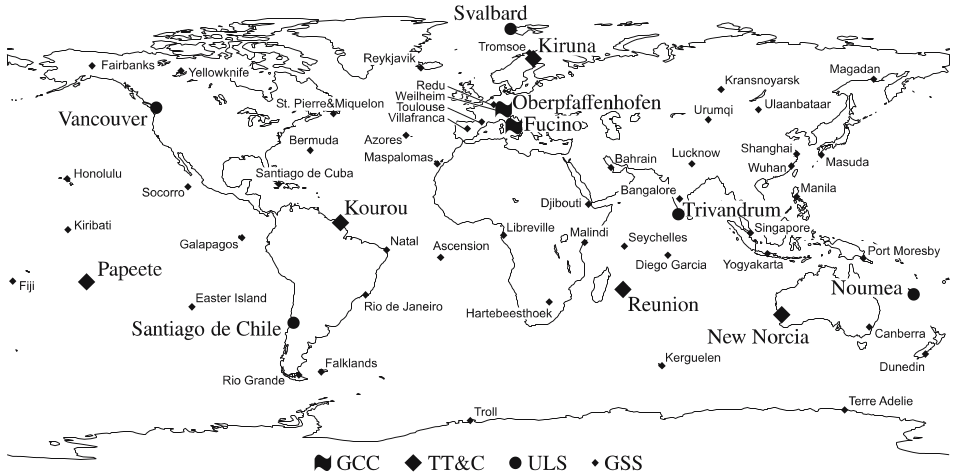
\includegraphics[width=0.9\columnwidth]{figures/galileo-ground-segment}
                \end{center}
            \end{figure}
        \end{column}
    \end{columns}

\end{frame}

\begin{frame}{BDS}

    \begin{itemize}
        \item Chinese network
        \vspace{0.2cm}
        \item Regional and global coverage
        \vspace{0.2cm}
        \item Composed by two systems: Beidou-1 and Beidou-2 (local and global coverage, respectively)
        \vspace{0.2cm}
        \item Orbit: MEO and GEO
        \vspace{0.2cm}
        \item Composed by 4 (Beidou-1) and 35 (Beidou-2) satellites
        \vspace{0.2cm}
        \item Operational in 2000 (Beidou-1) and 2020 (Beidou-2)
    \end{itemize}

\end{frame}

\begin{frame}{QZSS}

    \begin{columns}[t]
        \begin{column}[t]{0.4\textwidth}
            \begin{itemize}
                \item Japanese network
                \vspace{0.2cm}
                \item Regional network (limited to Japan)
                \vspace{0.2cm}
                \item Composed by four satellites
                \vspace{0.2cm}
                \item Orbit: GEO and quasi-zenith
            \end{itemize}
        \end{column}
        \begin{column}[t]{0.6\textwidth}
            \begin{figure}[!ht]
                \begin{center}
                    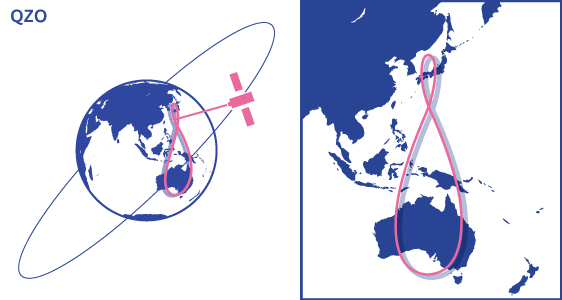
\includegraphics[width=0.9\columnwidth]{figures/qzss-orbit}
                \end{center}
            \end{figure}
        \end{column}
    \end{columns}

\end{frame}

\begin{frame}{IRNSS}

    \begin{columns}[t]
        \begin{column}[t]{0.4\textwidth}
            \begin{itemize}
                \item Indian network
                \vspace{0.2cm}
                \item Regional network (limited to India)
                \vspace{0.2cm}
                \item Composed by seven satellites
            \end{itemize}
        \end{column}
        \begin{column}[t]{0.6\textwidth}
            \begin{figure}[!ht]
                \begin{center}
                    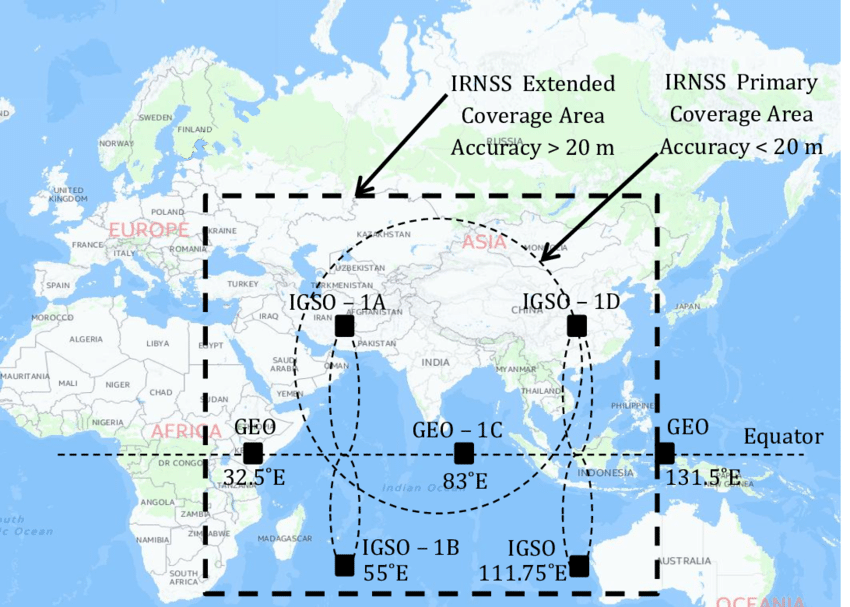
\includegraphics[width=0.9\columnwidth]{figures/irnss}
                \end{center}
            \end{figure}
        \end{column}
    \end{columns}

\end{frame}

\begin{frame}{Comparison Between Systems}

\begin{table}[!ht]\tiny
    \centering
    \begin{tabular}{lC{1cm}C{1cm}C{1cm}C{1cm}C{1cm}C{1cm}C{1cm}}
        \toprule[1.5pt]
        \multirow{2}{*}{\textbf{Characteristic}} & \multicolumn{7}{c}{\textbf{Network}} \\
                                                 & \textbf{GPS} & \textbf{GLONASS} & \textbf{Galileo} & \textbf{BDS} & \textbf{QZSS} & \textbf{IRNSS} & \textbf{KPS} \\
        \midrule
        Coverage      & Global        & Global      & Global         & Global      & Regional    & Regional    & Regional \\
        Country       & United States & Russia      & European Union & China       & Japan       & India       & South Korea\\
        Satellites    & 32            & 24          & 30             & 30          & 4           & 7           & 3 \\
        Orbit         & MEO           & MEO         & MEO            & MEO         & GEO         & GEO/MEO     & LEO \\
        Altitude [km] & 20200         & 19100       & 23200          & 21000       & 39000       & 36000       & 1000 \\
        Bands         & L1, L2, L5    & L1, L2      & E1, E5a, E5b   & B1, B2, B3  & L1, L2C, L5 & L5, S       & K \\
        Launch year   & 1978          & 1982        & 2016           & 2000        & 2010        & 2013        & 2021 \\
        Accuracy [m]  & 5-10          & 5-10        & 1-5            & 5-10        & 1-5         & 5-10        & 5-10 \\
        Status        & Operational   & Operational & Operational    & Operational & Operational & Operational & Planned \\
        \bottomrule[1.5pt]
    \end{tabular}
    \label{tab:networks-comparison}
\end{table}

\end{frame}

\begin{frame}{Experimental Networks}

    \begin{columns}[t]
        \begin{column}[t]{0.4\textwidth}
            \begin{itemize}
                \item Trust Point
                \vspace{0.3cm}
                \item Xona Space Systems
            \end{itemize}
        \end{column}
        \begin{column}[t]{0.6\textwidth}
            \begin{figure}[!ht]
                \begin{center}
                    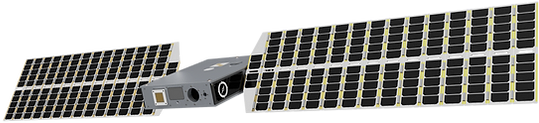
\includegraphics[width=0.9\columnwidth]{figures/xona-satellite}
                \end{center}
            \end{figure}
        \end{column}
    \end{columns}

\end{frame}

\begin{frame}{Remarks}

    \begin{itemize}
        \item So far, no other doctoral theses on this topic are known
        \vspace{0.3cm}
        \item here are already commercial initiatives aimed at deploying private GNSS networks using small satellites, but there is no fully operational network yet
        \vspace{0.3cm}
        \item The use of modulations such as LoRa and/or the use of chip-scale atomic clocks for applications of this type is also unknown
    \end{itemize}

\end{frame}
